% L22eqv.tex
% $Author$ $Date$

% \section{Invariant solutions of a small system-size KS}
% \label{sec:L22}
% Predrag created file              jul  9 2006

We now turn to exploring Hopf's vision
numerically, on a specific \KS\ system.
An instructive example is offered by the dynamics for
the  $L=22$  system
that we specialize to for the rest of this paper.
The size of this
small system is $\sim 2.5$ mean wavelengths
($\tildeL/\sqrt{2}= 2.4758$),
    \PC{define this $\sqrt{2}$ in the theory
        section, refer to it here
        }
and the competition between wavenumbers 2 and 3 states
leads to the empirically observed `sustained turbulence'.
Asymptotic attractor structure of small systems like
the one studied here
is very sensitive to system parameter variations, and,
as is true of
any realistic unsteady flow, there is no rigorous way of
establishing that this `turbulence' is sustained for all time,
rather than being
merely a very long transient on a way to an
attracting periodic state.
For large system size, as the one shown in \reffig{f:ks_largeL}, it is
hard to imagine a scenario under which attractive periodic states
(as shown in \refref{FSTks86} they do exist) would have significantly
large immediate basins of attraction.
Regardless of the
(non)existence of a $t \to \infty$ chaotic attractor, study
of the invariant unstable solutions and the associated Smale
horseshoe structures in system's \statesp\ offers valuable
insights into the observed unstable `coherent structures.'

Because of the strong $k^4$ contraction, for a small system size
one expects that the long-time dynamics is confined to low-dimensional
center manifold. Indeed, numerically the leading Lyapunov exponents of the
$L=22$ chaotic attractor are
$(\Lyap_i) = (0.048, 0, 0, -0.003, -0.189, -0.256, -0.290, \cdots)$,
so the chaotic dynamics mostly takes
place close to a 4-dimensional manifold, with strong
contraction in other dimensions.  The two zero exponents
are due to the
time and space translational symmetries of the \KSe,
and it was shown in \refrefs{Christiansen:97,LanCvi07}
that within particular curvilinear coordinate frames, the
dynamics on the attractor can sometimes be reduced to
local 1- or 2-dimensional maps.
Hence a relatively small
number of Fourier modes truncations, of order of $d \sim 10^2$
for the system studied here, suffices to obtain
numerically accurate (within $10^{-5}$) invariant
solutions.
% be significant for the dynamics, while the
% rest are in the numerical noise.
\PC{dropped ``See Figure~6 in \refref{Christiansen:97}.''}


We next investigate the properties of \eqva\ and \reqva\ and a large set
of the short periods \rpo s for KS in a periodic cell of
size $L=22$.
%\PC{we have not proven ``all" part}

\section{\Eqva\ and \reqva for L=22}

In addition to the trivial \eqv\ $u=0$ (denoted \EQV{0}),
we find three \eqva\ with dominant wavenumber $k$
(denoted \EQV{k}) for $k = 1, 2, 3$.  All {\eqva}, shown in
Fig.~\ref{f:KS22Equil}, are symmetric with respect to the reflection
symmetry \refeq{KSparity}.
In addition, \EQV{2} and \EQV{3} are symmetric with respect
to translation \refeq{KSshift}, by $L/2$ and $L/3$, respectively.
\EQV{2} and \EQV{3} essentially lie, respectively, in
the 2$^\mathrm{nd}$ and 3$^\mathrm{rd}$ Fourier component complex plane,
with small deformations from \ESedit{$k=2j$, $k=3j$} harmonics.

%
%%%%%%%%%%%%%%%%%%%%%%%%%%%%%%%%%%%%%%%%%%%%%%%%%%%%%%%%%%%%%%%%%%
\begin{figure}[t]
\begin{center}
  (a)\!\!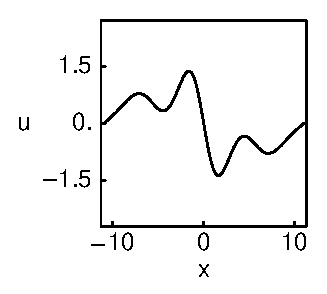
\includegraphics[width=0.35\textwidth]{figs/1wKS22equil.eps}
~~(b)\!\!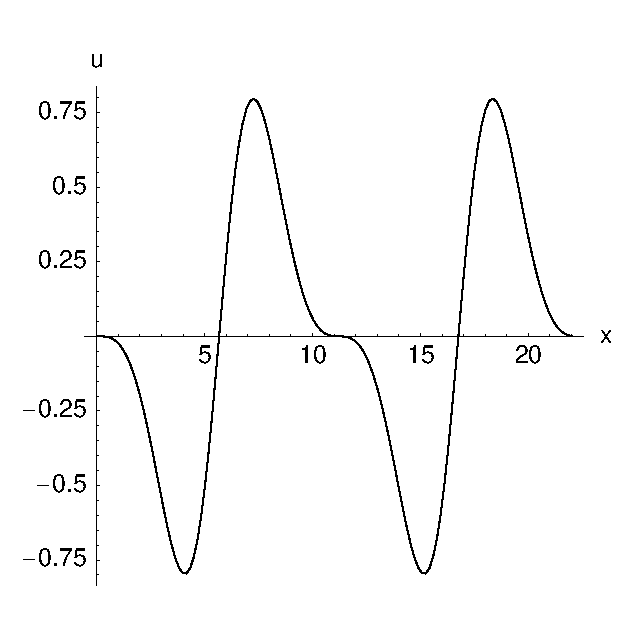
\includegraphics[width=0.35\textwidth]{figs/2wKS22equil.eps}
\\
  (c)\!\!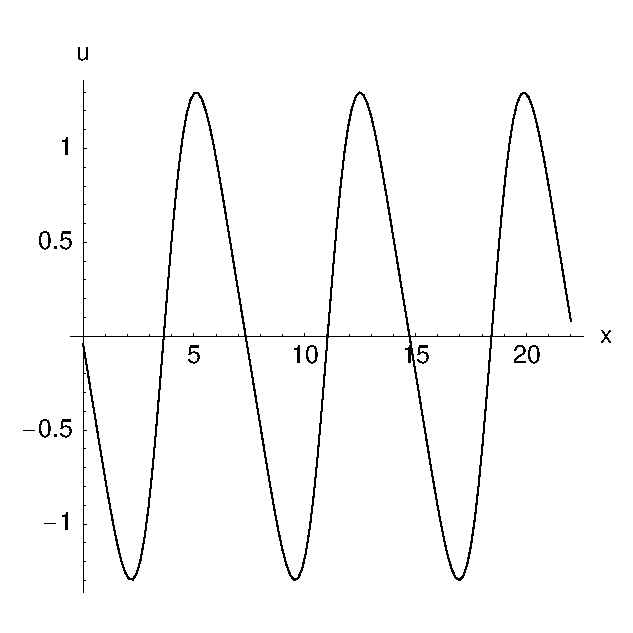
\includegraphics[width=0.35\textwidth]{figs/3wKS22equil.eps}
~~(d)\!\!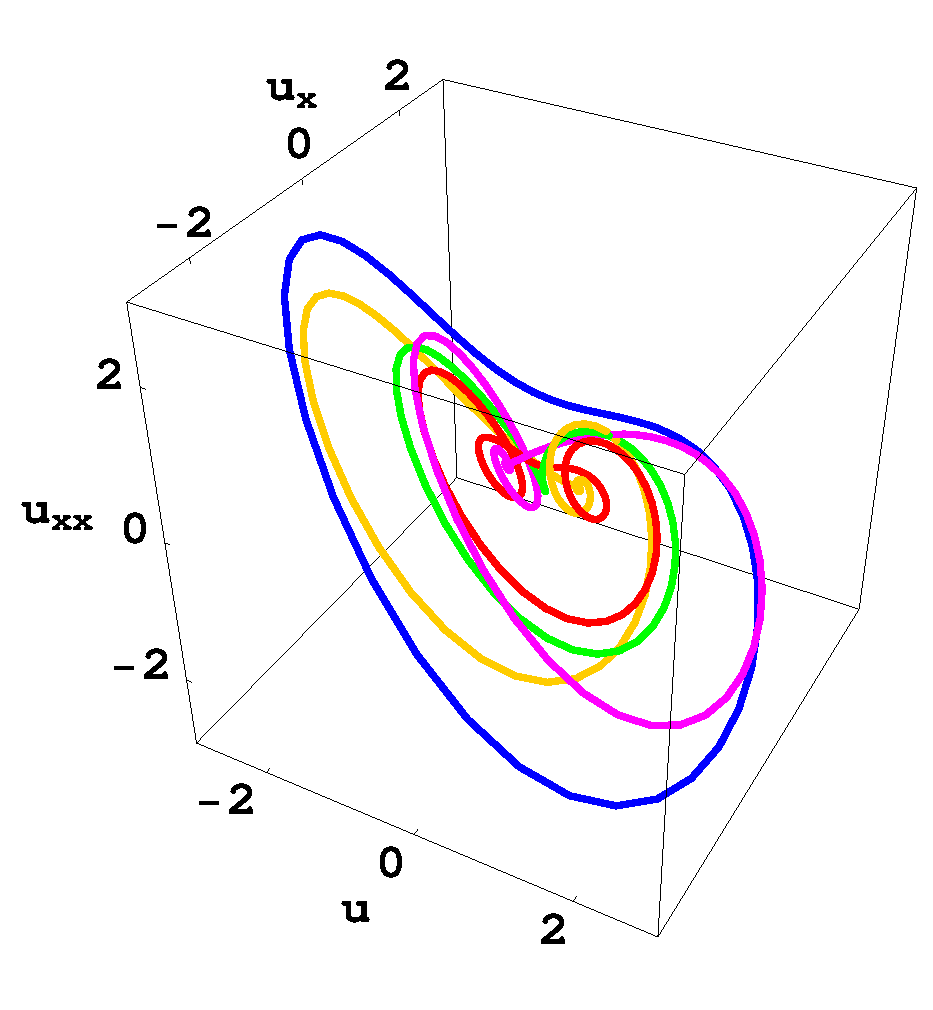
\includegraphics[width=0.35\textwidth]{figs/equilSpatial.eps}
\end{center}
\caption{
(a) \EQV{1}, (b) \EQV{2}, and (c)
\EQV{3} \eqva. The \EQV{0} \eqv\ is the $u(x)=0$
solution.
(d) $(u,u_x,u_{xx})$ representation
of (red) \EQV{1}, (green) \EQV{2},  (blue) \EQV{3} \eqva,
(purple) \REQV{+}{1},  and (orange) \REQV{-}{1} \reqva.
$L=22$ system size.
%, $N=64$ complex modes truncation.
    }
\label{f:KS22Equil}
\end{figure}
%%%%%%%%%%%%%%%%%%%%%%%%%%%%%%%%%%%%%%%%%%%%%%%%%%%%%%%%%%%%%%%%

The stability of the {\eqva} is characterized by the eigenvalues
$\eigExp[j]$ of the \stabmat.  The leading 10 eigenvalues for each
\eqv\ are listed in \reftab{tab:Eksym}. We compute (available upon request)
the corresponding eigenvectors as well. As an \eqv\ with $\mathrm{Re}
\lambda_j > 0$ is unstable in the direction of the corresponding
eigenvector $\jEigvec{j}$, the eigenvectors provide flow-intrinsic
(PDE discretization independent) coordinates which we use for visualization
of unstable manifolds and homo- / hetero-clinic connections between
\eqva.

% \begin{table}[t]\label{tab:EkEigs}
% \begin{center} \footnotesize
% \caption{ Eigenvalues of the \eqva\ for $L=22$.}
% \begin{tabular}{cccc} \hline
%   \EQV{0}  &    \EQV{1}        &    \EQV{2}        &  \EQV{3}   \\\hline
%   $0.2198$ &  $0.1308+i0.3341$ &  $0.1390+i0.2384$ &  $0.0933$\\
%   $0.2198$ &  $0.1308-i0.3341$ &  $0.1390-i0.2384$ &  $0.0933$\\
%   $0.1952$ &  $0.0824+i0.3402$ &  $0$              &  $0$\\
%   $0.1952$ &  $0.0824-i0.3402$ & $-0.0840+i0.1602$ & $-0.4128$\\
%   $0.0749$ &  $0$              & $-0.0840-i0.1602$ & $-0.6108+i0.3759$\\
%   $0.0749$ & $-0.2287+i0.1963$ & $-0.1194$         & $-0.6108-i0.3759$\\
%  $-0.3981$ & $-0.2287-i0.1963$ & $-0.2711+i0.3563$ & $-0.6108+i0.3759$\\
%  $-0.3981$ & $-0.2455$         & $-0.2711-i0.3563$ & $-0.6108-i0.3759$\\
%  $-2.1191$ & $-2.0554$         & $-2.0130$         & $-1.6641$\\
%  $-2.1191$ & $-2.0619$         & $-2.0378$         & $-1.6641$\\\hline
% \end{tabular}
% \end{center}
% \end{table}

The eigenvalues of \EQV{0} are determined by the linear part of the KS
equation \refeq{expanMvar}: $\lambda_k=(k/\tilde{L})^2-(k/\tilde{L})^4$.
For $L=22$, there are three pairs of unstable eigenvalues, corresponding,
in decreasing order, to three unstable modes $k=2,3$, and 1.  For each
mode, the corresponding eigenvectors lie in the plane spanned by
$\Re \, a_k$ and $\Im \, a_k$. \refTab{tab:Eksym}
lists the symmetries of the stability eigenvectors of
\eqva\ \EQV{1} to \EQV{3}.

\begin{figure}[t]
\begin{center}
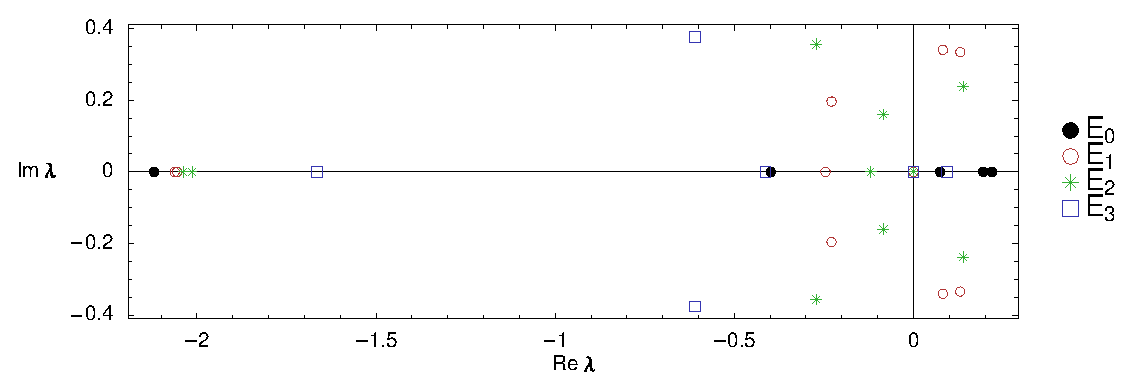
\includegraphics[width=4in]{figs/L22-eqvaEigenvalues.eps}
\end{center}
\caption{
Leading  \eqv\ stability eigenvalues,
$L=22$ system size.
%(b) Eigenvalues of \eqva\ and \reqva\ within
%the symmetric subspace $R_1$.
}
\label{f:KS22EkEigs}
\end{figure}

\begin{table}[t]
\caption{
Leading eigenvalues
$\eigExp[j]= \eigRe[j] \pm i\eigIm[j]$
and symmetries of the corresponding eigenvectors
of KS {\eqva} and \reqva\ for $L = 22$ system size.
We have used as our reference states the ones that lie within
the antisymmetric subspace  $\bbU^+$,
and also listed the symmetries of
the $L/4$ translated ones.
        }\label{tab:Eksym}
\begin{center} \footnotesize
\begin{tabular}{ccccc}
\EQV{1}& $\eigRe[j]$ & $\eigIm[j]$ & Symmetry & $\Shift_{1/4}\EQV{n}$ Symmetry\\\hline
  $\eigExp[1,2]$ & $0.1308$& $0.3341$ & -  & -\\
  $\eigExp[3,4]$ & $0.0824$& $0.3402$ & $\bbU^+$  & $\bbU^{(1)}$\\
  $\eigExp[5]$   & $0$     &          & -  & -\\
  $\eigExp[6,7]$ &$-0.2287$& $0.1963$ & $\bbU^+$  & $\bbU^{(1)}$\\
  $\eigExp[8]$   &$-0.2455$&          & -  & -\\
  $\eigExp[9]$   &$-2.0554$&          & $\bbU^+$  & $\bbU^{(1)}$\\
  $\eigExp[10]$  &$-2.0619$&          & -  & -\\\hline
\EQV{2}&  &  & \\\hline
  $\eigExp[1,2]$ & $0.1390$ & $0.2384$ & $\bbU^+$         & $\bbU^{(1)}$\\
  $\eigExp[3]$   & $0$      &          & $\Shift_{1/2}$        & $\Shift_{1/2}$\\
  $\eigExp[4,5]$ &$-0.0840$ & $0.1602$ & $\bbU^{(1)}$           & $\bbU^+$\\
  $\eigExp[6]$   &$-0.1194$ &          & $\Shift_{1/2}$        & $\Shift_{1/2}$\\
  $\eigExp[7,8]$ &$-0.2711$ & $0.3563$ & $\bbU^+,\,\bbU^{(1)},\,\Shift_{1/2}$  & $\bbU^+,\,\bbU^{(1)},\,\Shift_{1/2}$\\
  $\eigExp[9]$   &$-2.0130$ &          & $\bbU^{(1)}$           & $\bbU^+$\\
  $\eigExp[10]$  &$-2.0378$ &          & $\bbU^+$         & $\bbU^{(1)}$\\\hline
\EQV{3}&  &  & \\\hline
  $\eigExp[1]$   &$0.0933$  &          & $\bbU^+$     & $\bbU^{(1)}$\\
  $\eigExp[2]$   &$0.0933$  &          & -         & -  \\
  $\eigExp[3]$   &$0$       &          & $\Shift_{1/3}$    & $\Shift_{1/3}$\\
  $\eigExp[4]$   &$-0.4128$ &          & $\bbU^+,\,\Shift_{1/3}$  & $\bbU^{(1)},\,\Shift_{1/3}$\\
  $\eigExp[5,6]$ &$-0.6108$ & $0.3759$ & $\bbU^+$     & $\bbU^{(1)}$\\
  $\eigExp[7,8]$ &$-0.6108$ & $0.3759$ & -         & -\\
  $\eigExp[9]$   &$-1.6641$ &          & -         & -\\
  $\eigExp[10]$  &$-1.6641$ &          & $\bbU^+$     & $\bbU^{(1)}$ \\\hline
$\REQV{\pm}{1}$&  &  & \\\hline
  $\eigExp[1,2]$ & $0.1156$ & $0.8173$ & -  & -\\
  $\eigExp[3,4]$ & $0.0337$ & $0.4189$ & -  & -\\
  $\eigExp[5]$   & $0$      &          & -  & -\\
  $\eigExp[6]$   &$-0.2457$ &          & -  & -\\
  $\eigExp[7,8]$ &$-0.3213$ & $0.9813$ & -  & -\\\hline
$\REQV{\pm}{2}$&  &  & \\\hline
  $\eigExp[1]  $ & $0.3370$ &          & -  & -\\
  $\eigExp[2]  $ & $0$      &          & -  & -\\
  $\eigExp[3,4]$ &$-0.0096$ & $0.6288$ & -  & -\\
  $\eigExp[5,6]$ &$-0.2619$ & $0.5591$ & -  & -\\
  $\eigExp[7,8]$ &$-0.3067$ & $0.0725$ & -  & -\\
\end{tabular}
\end{center}
\end{table}

% % \subsection{\Reqva}
% \PC{
%     \refTab{tab:Eksym}:
%     replace D(m) by $\tau_{1/m}$  (?),
%     \\
%     $A(L/4)\EQV{n}$ symmetry by $\tau_{1/4}\EQV{n}$ (?)
%     \\
%     link caption to equations in symmetry section
%    }
% In addition to the \eqva, the KS system has pairs of
% \reqva\ \refeq{reqva} with fixed profiles
% moving at constant speed $\pm c$, \ie,
% \PCedit{ $u(x - ct,t)$, so they travel to the right for $c>0$ }
% \[
% u(x \PCedit{-} ct,t) = u(x, 0)\,.
% % \quad t \in \mathbb{R}\,.
% \]


    \PublicPrivate{%
        }{% switch to Private:
\begin{table}[t]    
\caption{
\PCedit{Experimental layout of \reftab{tab:Eksym} symmetries
        (incomplete, just testing the layout).
Need a rational way to label symmetries. The main thing we care about is
whether eigenvector is in $\bbU^-$, in which case its global continuation
remains within $\bbU^-$.
        }
        }\label{tab:EksymTEMP}
\begin{center} \footnotesize
\begin{tabular}{lccccc}
      && $\eigRe[j]$ & $\eigIm[j]$ & ~~~\Refl & $\Shift_{1/2}$\\
\EQV{2}&& &  & \\\hline
 &$\eigExp[1,2]$ & $~0.1390$ & $0.2384$ & $\Refl_1$         & $\bbU^-$\\
 &$\eigExp[3]$   & $0$      &          & $\Shift_{1/2}$        & $\Shift_{1/2}$\\
 &$\eigExp[4,5]$ &$-0.0840$ & $0.1602$ & $\bbU^-$           & $\Refl_1$\\
 &$\eigExp[6]$   &$-0.1194$ &          & $\Shift_{1/2}$        & $\Shift_{1/2}$\\
 &$\eigExp[7,8]$ &$-0.2711$ & $0.3563$ & $\Refl_1,\,\bbU^-,\,\Shift_{1/2}$  & $\Refl_1,\,\bbU^-,\,\Shift_{1/2}$\\
 &$\eigExp[9]$   &$-2.0130$ &          & $\bbU^-$           & $\Refl_1$\\
 &$\eigExp[10]$  &$-2.0378$ &          & $\Refl_1$         & $\bbU^-$\\
\EQV{3}&&  &  & \\\hline
 &$\eigExp[1]$   &$~0.0933$  &          & $\Refl_1$     & $\bbU^-$\\
 &$\eigExp[2]$   &$~0.0933$  &          & -         & -  \\
 &$\eigExp[3]$   &$0$       &          & $\Shift_{1/3}$    & $\Shift_{1/3}$\\
 &$\eigExp[4]$   &$-0.4128$ &          & $\Refl_1,\,\Shift_{1/3}$  & $\bbU^-,\,\Shift_{1/3}$\\
 &$\eigExp[5,6]$ &$-0.6108$ & $0.3759$ & $\Refl_1$     & $\bbU^-$\\
 &$\eigExp[7,8]$ &$-0.6108$ & $0.3759$ & -         & -\\
\end{tabular}
\end{center}
\end{table}
    } %end \PublicPrivate{%


%%%%%%%%%%%%%%%%%%%%%%%%%%%%%%%%%%%%%%%%%%%%%%%%%%%%%%%%%%%%%%%%%%
\begin{figure}[t]
\begin{center}
\includegraphics[width=0.3\textwidth]{figs/ks22_TW1_profile.eps}
\includegraphics[width=0.3\textwidth]{figs/ks22_TW2_profile.eps}\\
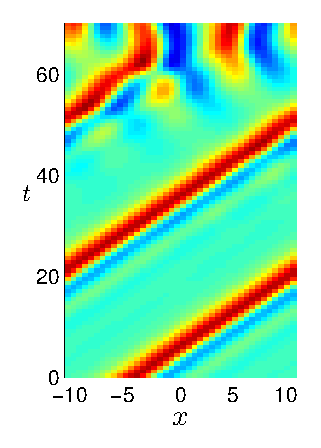
\includegraphics[width=0.3\textwidth]{figs/ks22_TW1_orbit_c.eps}
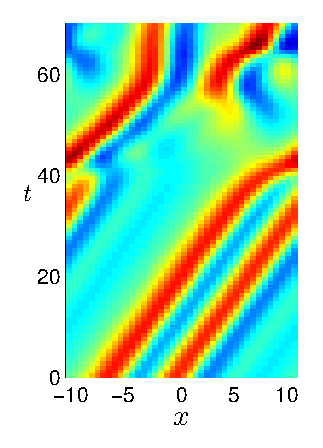
\includegraphics[width=0.3\textwidth]{figs/ks22_TW2_orbit_c.eps}
\end{center}
\caption{
% (a) \Reqv\ \REQV{+}{1}.
% with $L = 22$.
% (b) \Reqv\  \REQV{+}{2}.
\Reqva : \REQV{+}{1} with velocity $c = 0.737$ and \REQV{+}{2} with
velocity $c = 0.350$.
\REQV{+}{2} belongs to the bifurcation branch starting
at point $M$ in \PCedit{\reffig{fig:ksBifDiag}}.
The upper panels show the \reqva\ profiles.  The lower panels show
evolution of slightly perturbed \reqva\ and their decay into generic
turbulence. Each \reqv\ has a reflection symmetric partner related by
$u(x) \to -u(-x)$ travelling with velocity $-c$.
% , $c \to -c$.
} \label{f:ks22TW}
\end{figure}
%%%%%%%%%%%%%%%%%%%%%%%%%%%%%%%%%%%%%%%%%%%%%%%%%%%%%%%%%%%%%%%%%%

%\PC{ \refeq{f:ks22TW} top panel: remove velocity labels. }
%\PC{split ks22\_RE1-2.eps into four,
%    so \reffig{f:ks22TW} can be reformatted}
Consistent with the bifurcation diagram of \reffig{fig:ksBifDiag},
we find two pairs of \reqva\ \refeq{reqva} with velocities $c =\pm 0.73699$ and $\pm 0.34954$
which we label \REQV{\pm}{1} and \REQV{\pm}{2},
for `traveling waves'.
The profiles of the two \reqva\ and their time evolution
with eventual decay into the chaotic attractor are
shown in \reffig{f:ks22TW}.  The leading eigenvalues of
\REQV{\pm}{1} and \REQV{\pm}{2} are listed in \reftab{tab:Eksym};
those with $\eigRe > -2.5$ are also plotted in
\reffig{f:KS22EkEigs}.
\PC{ dropped this:
    ``The eigenvectors do not belong to any of the symmetric
    subspaces of {\KSe} discussed in \refsect{sec:KSeSymm}."
    }
%\PC{please list $c$ in \reftab{tab:TW} }
%\begin{table} \label{tab:TW}
%\caption{
%Stability eigenvalues of the \reqva\ for $L=22$.
%} %\ for $L=22$.}
%\begin{center} \footnotesize
%\begin{tabular}{ccc|ccc}
%  \multicolumn{3}{c}{$\REQV{\pm}{1}$ ~($c = \pm 0.73699$)}  &
%  \multicolumn{3}{c}{$\REQV{\pm}{2}$ ~($c = \pm 0.34954$)} \\\hline
%  &$\eigRe[j]$ & $\eigIm[j]$ & & $\eigRe[j]$ & $\eigIm[j]$\\
%  $\eigExp[1,2]$ & $0.1156$ & $0.8173$ & $\eigExp[1]  $ & $0.3370$ & \\
%  $\eigExp[3,4]$ & $0.0337$ & $0.4189$ & $\eigExp[2]  $ & $0$ & \\
%  $\eigExp[5]$   & $0$      &          & $\eigExp[3,4]$ &$-0.0096$ & $0.6288$\\
%  $\eigExp[6]$   &$-0.2457$ &          & $\eigExp[5,6]$ &$-0.2619$ & $0.5591$\\
%  $\eigExp[7,8]$ &$-0.3213$ & $0.9813$ & $\eigExp[7,8]$ &$-0.3067$ & $0.0725$\\
%\end{tabular}
%\end{center}
%\end{table}

\PCedit{
\refTab{tab:L22cminus} lists \eqv\ energy $E$,
the local Poincar\'e section return time $T$,
radially expanding Floquet multiplier $\ExpaEig_e$, and
the least contracting Floquet multiplier $\ExpaEig_c$
for all $L=22$ \eqva\ and \reqva.
The return time $T=2\pi/\eigRe[e]$ is given by the imaginary
part of the leading complex eigenvalue,
the expansion
multiplier per one turn of the most unstable spiral-out by
$\ExpaEig_e\approx\exp(\eigRe[e] T)$, and the contraction
rate along the slowest contracting stable eigendirection by
$\ExpaEig_c\approx\exp(\eigRe[c]T)$. We learn that the shortest
`turn-over' time is $\approx 10-20$, and that if there exist
horseshoe sets of unstable \po s associated with
these \eqva,  they have unstable
multipliers of order of $\ExpaEig_e \sim 5-10$, and that
they are surprisingly thin in the folding direction, with
contracting multipliers of order of 1-4\%, as in \refref{LanCvi07}.
        } %end \PCedit{

\begin{table}[h!]
    \caption{
    Properties of \eqva\ and \reqva\ determining
    the system dynamics in their vicinity.  $T$ is characteristic
    time scale of the dynamics, $\ExpaEig_e$ and $\ExpaEig_c$ are the
    expansion and contraction rates.
            }
\begin{center} \footnotesize
    \begin{tabular}{l|rrrr}
                 & $E$~~   & $T$~~  & $\ExpaEig_e$  & $\ExpaEig_c$  \\ \hline
 $\EQV{1}\ $     &\ 0.2609 &\ 18.81 &\ 4.79     &\ 0.04 \\
 $\EQV{2}\ $     &\ 0.4382 &\ 26.35 &\ 5.99     &\ 0.03 \\
 $\EQV{3}\ $     &\ 1.5876 &\ 10.71 &\ 9.92     &\ 0.01 \\
 $\REQV{\pm}{1}$ &\ 0.4649 &  &  & \\
 $\REQV{\pm}{2}$ &\ 0.6048 &  &  & \\
    \end{tabular}
\end{center}
\label{tab:L22cminus}
\end{table}

\subsection{Unstable manifolds of \eqva\ and their heteroclinic
            connections}
\label{sec:unstMnflds}

In this section we explore the structure of unstable
manifolds of the {\eqva}.  As shown in \refTab{tab:Eksym},
the \EQV{1} \eqv\ has two unstable
planes within which the solutions are spiralling out (\ie, two
pairs of complex conjugate eigenvalues).  The \EQV{2} has one such plane,
while the \EQV{3} has two real positive eigenvalues, so the solutions are
moving radially away from the \eqv\ within the plane spanned
by the corresponding eigenvectors.  Since \EQV{1} has
a larger unstable subspace, it is expected to have much less influence on the
long time dynamics compared to \EQV{2} and \EQV{3}.

\begin{figure}[t]
\begin{center}
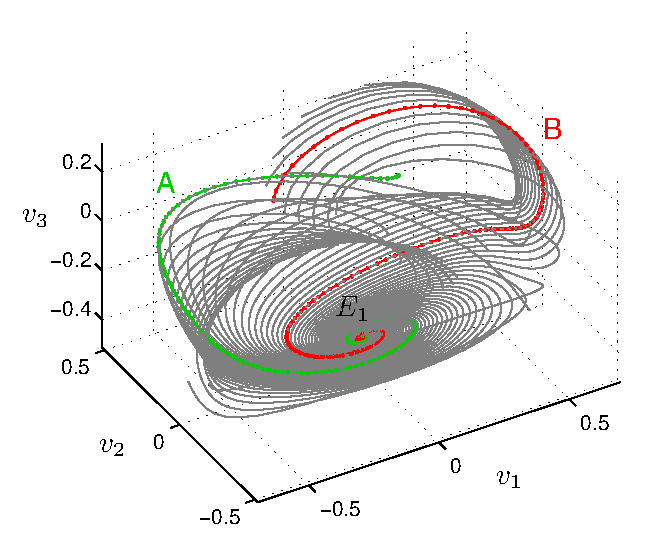
\includegraphics[width=0.5\textwidth]{figs/ks22_E1_plane1_manifold_c.eps}
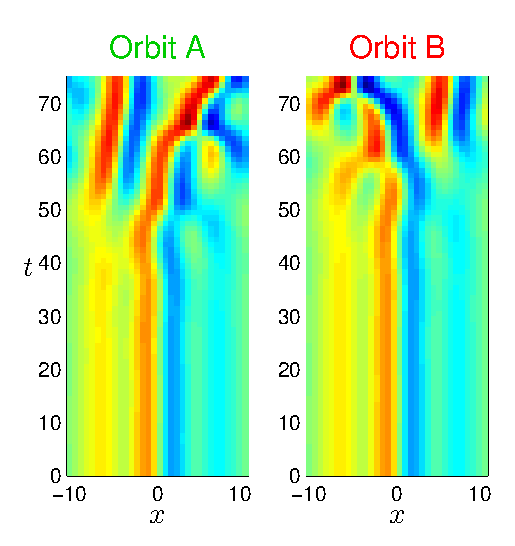
\includegraphics[width=0.4\textwidth]{figs/ks22_E1_plane1_orbits_c.eps}
\end{center}
\caption{
The left panel shows the unstable
manifold of \eqv\ \EQV{1} starting within the plane
corresponding to the first pair of unstable eigenvalues. The
coordinate axes $v_1$, $v_2$, and $v_3$ are constructed from vectors
$\Re \,\jEigvec{1}$, $\Im \,\jEigvec{1}$,
and $\Re \,\jEigvec{6}$
by Gram-Schmidt orthogonalization.
The right panel shows spatial representation of two orbits $A$ and $B$.
The change of color from blue to red indicates increasing values of
$u(x)$.
}
\label{f:KS22E1man1}
\end{figure}

To construct an invariant manifold containing solutions
corresponding to the pair of unstable complex conjugate eigenvalues,
$\eigExp = \eigRe \pm i\eigIm$,
$\eigRe > 0$, we start with a set of
initial conditions near \eqv\ \EQV{k},
\beq
  a(0) = a_{{\EQV{k}}} + \epsilon\,\exp(\delta)\jEigvec{j}
\,,
\ee{linUnstMan}
where $\delta$ takes the set of values uniformly distributed in the
interval $[0,2\pi\eigRe/\eigIm]$, $\jEigvec{j}$ is a unit vector in the
unstable plane, and $\epsilon > 0$ is small.

\begin{figure}[t]
\begin{center}
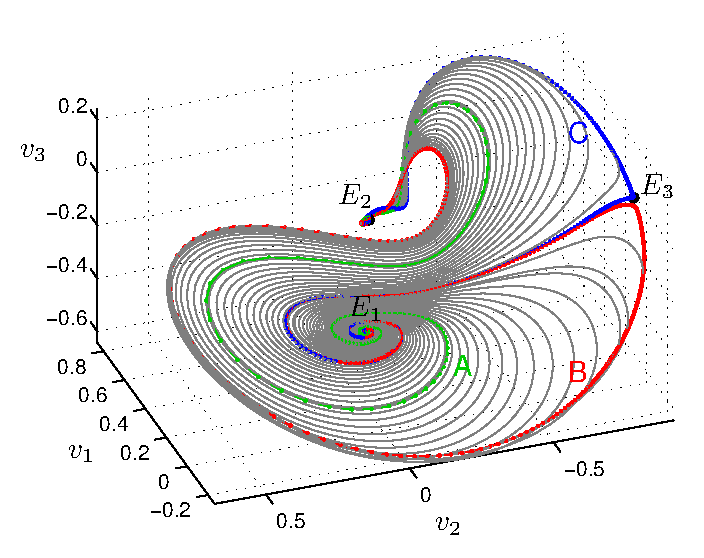
\includegraphics[width=0.48\textwidth]{figs/ks22_E1_plane2_manifold_c.eps}
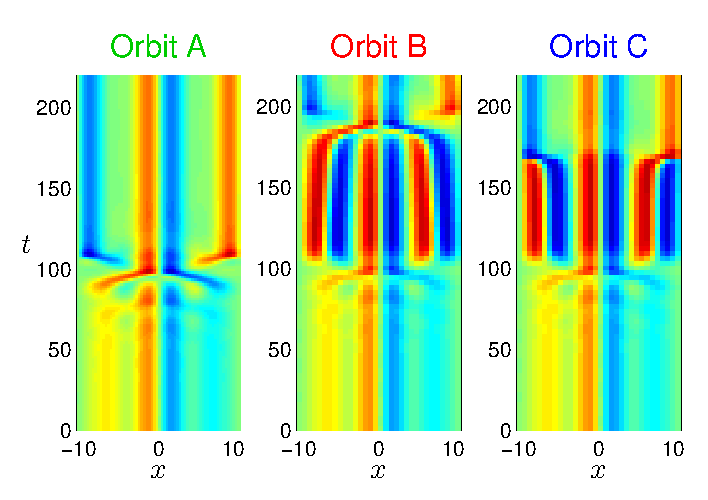
\includegraphics[width=0.48\textwidth]{figs/ks22_E1_plane2_orbits_c.eps}
\end{center}
\caption{
The left panel shows the unstable
manifold of \eqv\ \EQV{1} starting within the plane
corresponding to the second pair on unstable eigenvalues. The
coordinate axes $v_1$, $v_2$, and $v_3$ are constructed from vectors
\Re\, $\jEigvec{3}$, \Im\, $\jEigvec{3}$, and \Re\, $\jEigvec{6}$
by Gram-Schmidt orthogonalization.
The right panel shows spatial representation of three orbits. Orbits
$B$ and $C$ pass close to the \eqv\ \EQV{3}.
   }
\label{f:KS22E1man2}
\end{figure}

The manifold starting within the first unstable plane of \EQV{1}, with
eigenvalues $0.1308\pm i\,0.3341$, is shown in
\reffig{f:KS22E1man1}. It appears to fall directly into the
chaotic attractor.  The behavior of the manifold starting within
the second unstable plane of \EQV{1}, eigenvalues $0.0824\pm i \, 0.3402$, is
remarkably different: as can be seen in \reffig{f:KS22E1man2},
all orbits within the manifold converge to the \eqv\ \EQV{2}.  The
manifold also contains a heteroclinic connection from \EQV{1} to \EQV{3},
and is bordered by the $\eigExp[1]$ unstable manifold of \EQV{3}.
\PC{explain how this is due to symmetry, explicit reference to Kevrekidis}

\begin{figure}[h]
\begin{center}
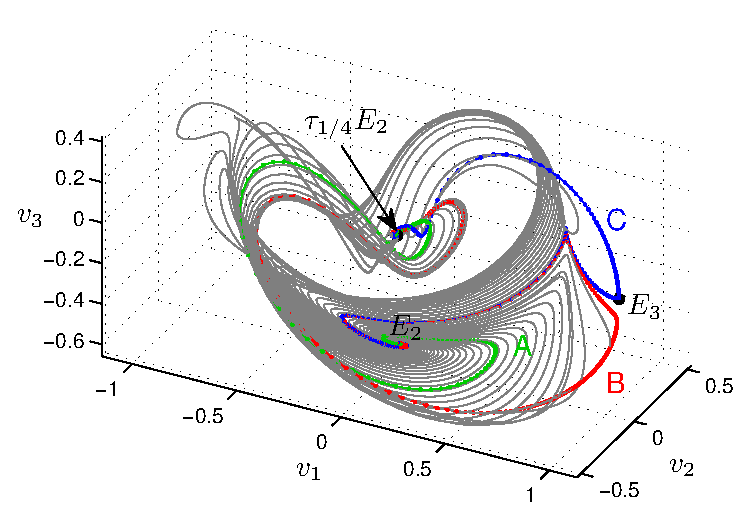
\includegraphics[width=0.48\textwidth]{figs/ks22_E2_manifold_c.eps}%
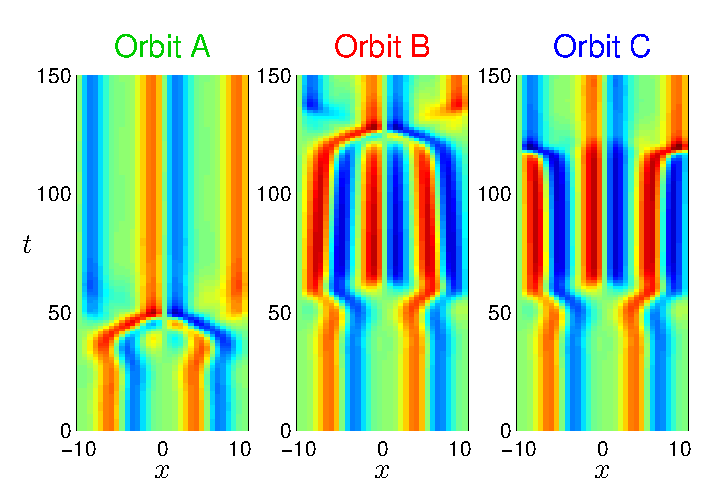
\includegraphics[width=0.48\textwidth]{figs/ks22_E2_orbits_c.eps}
\end{center}
\caption{
The left panel shows the two-dimensional
unstable manifold of \eqv\ \EQV{2}. The coordinate axes
$v_1$, $v_2$, and $v_3$ are constructed from vectors
\Re\, $\jEigvec{1}$, \Im\, $\jEigvec{1}$, and $\jEigvec{7}$
by Gram-Schmidt orthogonalization.
The right panel shows spatial representation of three orbits. Orbits
$B$ and $C$ pass close to the \eqv\ \EQV{3}. See
\reffig{f:KS22Manifold} for a different visualization.
       }
\label{f:KS22E2man}
\end{figure}


%%%%%%%%%%%%%%%%%%%%%%%%%%%%%%%%%%%%%%%%%%%%%%%%%%%%%%%%%%%%%%%%
\begin{figure}[t]
\begin{center}
%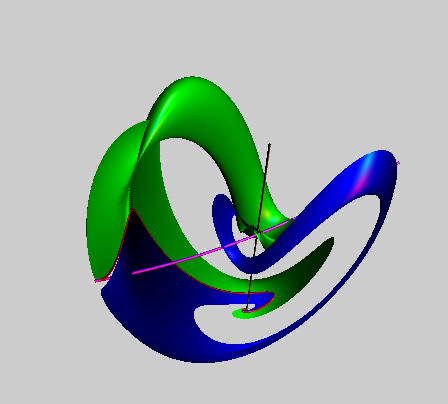
\includegraphics[width=0.6\textwidth]{figs/ks22manifold.ps}
(a) 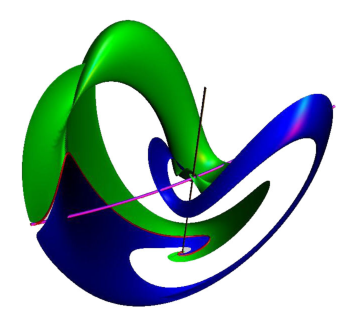
\includegraphics[height=2in]{figs/ks22manifold1.eps}
(b) \includegraphics[width=0.3\textwidth]%,origin=c]%
        {figs/ks22E2-E3hetero.eps}
\end{center}
\caption{
(a) (blue/green) The unstable manifold of \EQV{2}~\eqv.
%\ of KS equation for $\tilde{L}=3.5014$, N=64 mode truncation.
    (black line) The circle of \EQV{2}~\eqva\
related by the translation invariance.
(purple line) The circle  of \EQV{3}~\eqva.
(red) The heteroclinic connection
from the \EQV{2}~\eqv\ to the \EQV{3}~\eqv\ splits
the manifold into two parts,
colored (blue) and (green).  See
\reffig{f:KS22E2man} for a different visualization.
(b) \EQV{2}~\eqv\ to \EQV{3}~\eqv\ heteroclinic
connection. Here we omit the unstable manifold of \EQV{2},
keeping only a few neighboring trajectories in order to indicate
the unstable manifold of \EQV{3}. The \EQV{2} and \EQV{3}
families of \eqva\ arising from the continuous translational
symmetry of KS on a periodic domain are indicated by the two circles.
        }
\label{f:KS22Manifold}
\end{figure}
%%%%%%%%%%%%%%%%%%%%%%%%%%%%%%%%%%%%%%%%%%%%%%%%%%%%%%%%%%%%%%%%%%

\PC{
    \refFig{f:KS22Manifold}: projection base same as in the \reffig{f:KS22E2man}
    merge with \reffig{f:KS22unstM} into one figure.
   }
The two-dimensional unstable manifold of \EQV{2} is shown in
\reffig{f:KS22E2man}.  All orbits within the manifold converge
to \EQV{2} shifted by $L/4$.  So this manifold can be viewed as a homoclinic
connection.  It also contains a pair of heteroclinic connections from
\EQV{2} to \EQV{3}.

The \eqv\ \EQV{3} has a pair of real unstable eigenvalues
equal to each other.  Therefore, within the plane spanned by the
corresponding eigenvectors, the orbits move radially away from
the \eqv.  In order to trace out the unstable manifold,
we start with a set of initial conditions within the unstable plane
\beq
 a(0) = a_{{\EQV{3}}} + \epsilon(v_1 \cos \phi + v_2 \sin \phi)\,,
  \quad\phi\in[0,2\pi]\,,
\label{unsManSeed}
\eeq
where $v_1$ and $v_2$ are orthonormal vectors within the
plane spanned by the two unstable eigenvectors, seeded as in
\refeq{linUnstMan}.
  The unstable manifold
of \EQV{3} is shown in \reffig{f:KS22E3man}.  The 3-fold symmetry of
the manifold is related to the symmetry of \EQV{3} with respect to
translation by $L/3$.  The manifold contains heteroclinic orbits
connecting \EQV{3} to three different points of the continuum of {\eqva}
\EQV{2}
translated by 0 and $\pm L/6$.  Note that there are two different
heteroclinic orbits ($B$ and $C$) connecting \EQV{3} to the same point in the
\EQV{2} continuum.  Note also that the segments of orbits $B$ and $C$
between \EQV{3} and \EQV{2} in \reffigs{f:KS22E1man2}{f:KS22E2man}
represent the same heteroclinic connections as orbits $B$ and $C$ in
\reffig{f:KS22E3man}.

An understanding of the ubiquity of heteroclinic connections in KSe, as
opposed to a general high-dimensional system, is provided in \refref{KNSks90}.
For our system size one has to notice that there are exactly two representatives
of the $\EQV{2}$ family that lie in the intersection of $\bbU^+$ and $\bbU^{(1)}$ related
to each other by an $L/4$ shift. Denote them by $\EQV{2}$ and $\Shift_{1/4}\EQV{2}$. The unstable eigenplane of
$\EQV{2}$ lies on $\bbU^+$ while that of $\Shift_{1/4}\EQV{2}$ lies on $\bbU^{(1)}$, \cf\ \reftab{tab:Eksym}. 
The $\EQV{3}$ family members that live in $\bbU^+$ have one of their unstable eigenvectors (the one related to the heteroclinic
connection to $\EQV{2}$ family)  on $\bbU^+$, while the other does not lie on an invariant subspace.
Similarly, for the $\EQV{1}$ family we observe that the equilibria in $\bbU^+$ have
an unstable plane on $\bbU^+$ (again related to the heteroclinic connection) and a second one with no symmetry. 
%Since $\bbU^{+}$ is invariant under the \KS\ flow the unstable manifolds (or their subspaces
Thus $\Shift_{1/4}\EQV{2}$ appears as a sink on $\bbU^+$, while all other equilibria appear as sources.
This explains the heteroclinic connections from $\EQV{1}\,,\EQV{2}$ and $\EQV{3}$ to $\Shift_{1/4}\EQV{2}$.
Observing that $\Shift_{1/4} \bbU^+= \bbU^{(1)}$ and taking into account \reftab{tab:Eksym} we understand that on $\bbU^{(1)}$
we have connections from $\Shift_{1/4}\EQV{2}$ (and the members of $\EQV{1}$ and $\EQV{3}$ families) to $\EQV{2}$ and the
formation of a heteroclinic loop. Due to the translational invariance of KSe there is a heteroclinic loop for any two points
of the $\EQV{2}$ family related by an $L/4$-shift.

\begin{figure}[t]
\begin{center}
\includegraphics[width=0.45\textwidth]{figs/ks22_E3_manifold.eps}
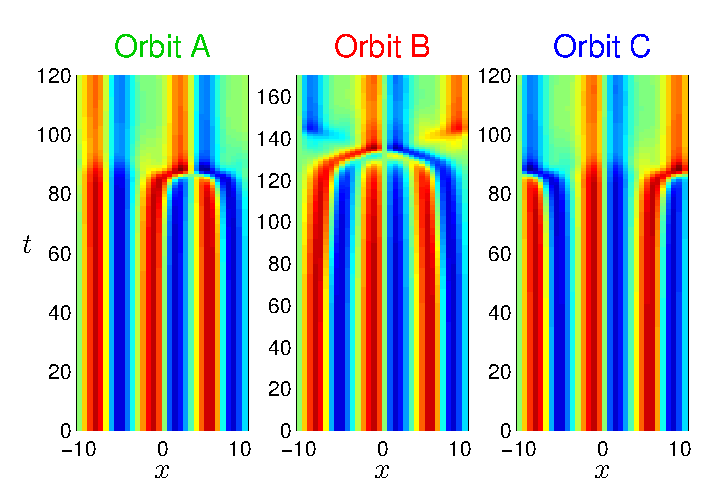
\includegraphics[width=0.5\textwidth]{figs/ks22_E3_orbits_c.eps}
\end{center}
\caption{
The left panel shows the two-dimensional
unstable manifold of \eqv\ \EQV{3}. The coordinate axes
$v_1$, $v_2$, and $v_3$ are constructed from vectors
$\jEigvec{1}$, $\jEigvec{2}$, and $\jEigvec{4}$ by Gram-Schmidt orthogonalization.
The black line shows a family of \EQV{2}~\eqva\ related by translational
symmetry. The right panel shows spatial representation of
three orbits. Orbits $B$ and $C$ are two different heteroclinic orbits
connecting \EQV{3} to the same point on the \EQV{2} line.
        }
\label{f:KS22E3man}
\end{figure}

%\PC{Check next what these 2 unstable eigenvectors for \EQV{3}~\eqv\ are
%    - when they are equal in magnitude you expect a `star',
%    all directions in their plane going straight out.
%    Do they all fall into \EQV{2}~\eqv?
%    }
